\chapter{Background}
\label{chap2}

\section{Robotic Manipulation}

In the present study, we consider the general research question: how should robots be programmed to manipulate (e.g. grasp) objects? 
There exist two common approaches to this problem in the robotics literature.
One approach is for a human expert to provide the robot with an analytical model of itself and its environment. 
Using this model, the robot achieves its manipulation goals in two phases: planning and execution.
%plans an end-effector trajectory and then executes that trajectory to perform the desired manipulation.
Planning is often performed in simulation using models of object geometry and robot/environment dynamics.
Once the robot has found a feasible plan, it then executes that plan via physical robot actuation.
One disadvantage to this approach is that due to imperfect precalculated dynamical models and robot calibration, executed manipulations can easily become unstable and fail \cite{dang2012tactile}.

%Another approach is to formulate the manipulation task as a control problem that utilizes force, torque, and tactile sensors to improve robustness.
Another approach is to remove the requirement of human-supplied models and have the models learned autonomously from data using statistical learning techniques.
The key advantages of this type of \emph{model-free} approach~\cite{Spall1998,hornung2014anomaly} are that apriori object and dynamical models are not required to succeed in the task; the model is learned automatically from data.
In this thesis, we define \emph{model-free} \cite{Spall1998} systems as those that function without given explicit knowledge of physics or geometry from human experts.
%As well, the robot is granted the capacity to adapt to unexpected changes in the environment.
%This results in a system that is more robust to pose uncertainties without complete dependence on detailed human-calculated environmental models \cite{dang2012tactile}.

%The latter approach is also closer to how the human motor system is known to function (see Section \ref{high_level_processes}).  
%There is ample physiology and neuroscience literature from which inspiration and insight to devising successful manipulation schemes can be drawn based on the human sensory system, with much success already attained \cite{felip2011emptying, leoni1998implementing, romano2011human, sikka1994tactile}.



\subsection{Model-free schemes}

%In this thesis, we define \emph{model-free} \cite{Spall1998} systems as those that function without given explicit knowledge of physics or geometry from human experts.
%Instead, the model is learned autonomously from data using a machine learning algorithms.
%Another approach to robotic manipulation in the literature is to analyze data compiled from a series of successful manipulations and extract features from the data that are indicative of successful manipulations.
%Once these features are acquired, they can then be used to predict success in future manipulations.

One example of such a learning technique is called the Self-Organizing Map (SOM), an architecture of Artificial Neural Networks (ANN) that spatially and uniformly organizes features automatically by input signals \cite{kohonen1990self}.
An example where SOMs have been used successfully is in \cite{steffen2007experience}: objects are grasped based on hand posture and tactile experience of previously successful grasps.
Experience is represented as a low dimensional smooth manifold in hand posture space. 
%, which is implemented as a SOM-variant.
%Successful grasps are used to continually update the SOM experience base that is then used to guide subsequent grasps to their closest matching posture in the experience base.
%Figure~\ref{fig:grasp_som} depicts the experience base graphically.

A similar system was devised in \cite{ratnasingam2011object}, where a SOM was used to map finger joint angles and tactile readings to object shape and size.
The system could identify previously grasped objects as well as categorize new objects as being a particular shape and size.
%The system successfully recognized 22 out of 25 different objects.

The same authors obtained similar results with another algorithm inspired by biological spiking neurons, called a spiking neural network \cite{ratnasingam2011spiking}.
For this scheme, joint angle input is encoded into a series of spike trains which result in three feature outputs that are then used to recognize and classify grasped objects.
In addition, similar objects tended to cluster in output feature space.
% Figure~\ref{fig:sensory_clustering}).
The authors' system was able to recognize objects of different shapes as well as objects with the same shape but different size.

In \cite{dang2011blind}, the authors present blind grasping: a novel approach to object grasping that does not require visual feedback or apriori 3D object models.
Their scheme works from a database of one thousand stable grasps from the Columbia Grasp Database using the model of a BarrettHand. 
Corresponding tactile feedback during grasps of objects simulated in the GraspIt! simulator are also recorded.
%Grasps are simulated in GraspIt!.
They proceed to create feature vectors comprising simulated tactile and robot kinematic data which they then use to train an SVM to classify grasps as being stable or unstable. 
%Figure~\ref{fig:tact_example} demonstrates such a feature vector as representing a stable grasp.
In this way, the system was able to learn tactile feedback indicative of a stable grasp.
%Once these successful tactile and kinematic features are learned, the robot hand can move its wrist and re-shape its hand to explore the object until similar tactile contacts to grasps in the database are achieved.

\subsection{Model-based schemes}

In \emph{model-based} schemes, a human expert provides the robot apriori models which, for example, map sensory input signals to specific control policies. 
This approach grants the advantage of providing the robot access to the understanding of the task dynamics of the researcher.
The disadvantage of this approach is that the supplied model may contain errors and is limited by the domain expertise of the researcher.
%would not generalize to aspects not specifically modeled.

In \cite{felip2011emptying}, the authors present sensor-based atomic controllers for a robotic hand/arm system to empty a box containing an undefined number of unknown objects.
Manipulation primitives are defined that search, grasp and transport objects from the box to predefined locations.
A finite state machine (FSM) is used to transition between motion primitives based on corresponding sensory feedback.
%This FSM is presented graphically in Figure~\ref{fig:grasp_fsm}.
The authors also compare a vision-plus-tactile-based version of their system to a purely tactile-based version.
They found that while the version which incorporated vision was more efficient at completing the empty-the-box manipulation task, the tactile version was also successful.
Vision was only crucial in determining if the box was empty; in the non-vision based system, a human moderator was required to tell the robot when it had finished its task.
The authors in \cite{felip2011emptying} also present an interesting scheme that compensates for errors in translation of the robotic hand.
The hand repositions itself if there is force experienced by only one finger, denoting a single hand/object contact.
The controller compensates by moving the hand in direction of single contact, which effectively repositions the manipulator above the object.

In~\cite{Lynch1999}, the authors take an analytical approach to the non-prehensile toppling task. 
This approach, while successful, assumes knowledge of the dynamics of the entire system and would therefore not generalize to operation outside of controlled factory environments where complete models of robot-object interaction dynamics were unavailable.
Another analytical approach to a non-prehensile tumbling task, given apriori models of how the system reacts to the robot at each phase of the task, is studied in~\cite{sawasaki1989tumbling}.

In \cite{Zhang2012}, an analytical approach is applied to the non-prehensile task of manipulating an object with rolling contacts across a robotic finger tip using tactile sensor feedback.
Their approach relies on accurate apriori kinematic and dynamic models of the robot and its environment.

\subsection{Human-inspired schemes}

%The human motor system is highly complex.
%Creating a robot hand with dexterous manipulation skills reaching human capabilities is no easy task.
In the human hand, there are a wide variety of receptors in the skin and muscles which in turn respond to a wide variety of stimuli.
Sensed phenomena include skin stretch, skin curvature, vibration and muscle force and length.
One baffling aspect of the human motor system however is that information bandwidths range from just a few Hz to possibly several hundred Hz.
In terms of technological performance, this is horrendously slow.
Information is also time varying, nonlinear, and its encoding scheme (known as pulse-frequency) obscures much of the raw inputs from the nerve endings.
How these deficiencies are made up for, however, is a high degree of parallelism and redundancy \cite{howe1993tactile}.

It is also known that the human motor system executes manpulations as a series of discrete states that transition based on afferent signals \cite{Johansson1984}.
Since this type of model is appropriate for execution on a computer, it has been quite popular to model the robotic grasping task as a Finite State Machine (FSM), which transitions between states base on tactile or other intrinsic contact input events \cite{leoni1998implementing, sikka1994tactile}.

%In \cite{howe1993tactile}, Howe presents a comprehensive overview of robotic hand systems in his 1993 review article.
%Howe's abstract design of robotic hands has since been left virtually unchanged \cite{cutkosky2008force}.
%Figure~\ref{fig:touch_sensors} shows a simplified schematic drawing of his design, which obtains inspiration from the physiology of the human hand.
%Not shown in Howe's diagram, however, is another popular fingertip sensor implementation based on calculating the deformation of a bag of fluid, as shown in Figure~\ref{fig:fingertip_sensors}.  

%FIGURE
%\begin{figure}[]
%	\centering
%	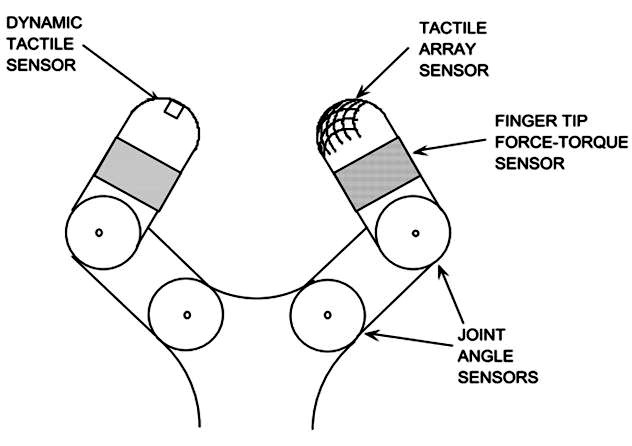
\includegraphics[width=\linewidth]{images/touch_sensors}
%	\caption{Schematic drawing of a robot hand with several types of contact sensors, reproduced from \cite{howe1993tactile}. Permission to reproduce is pending.}
%	\label{fig:touch_sensors}
%\end{figure}
%ENDFIGURE

The authors in \cite{leoni1998implementing} present an approach to tactile-motor coordination of a robotic hand based on a neurological model of the human tactile-motor system.
This model is implemented as a series of ANNs whose function and structure reflect discoveries in the human sensory areas specific to object grasping.
A scheme based on SOMs was chosen to model these sensory areas, since they must process a high rate of combined tactile and somatosensory input.
Use of the SOM controlled the volume of incoming inputs by making small, efficient adjustments to the model each time a new input vector became available.
%See Figure~\ref{fig:sensor_processing} for a graphical overview of their overall system.

The authors in \cite{romano2011human} developed a human-inspired robotic grasp controller that gently picks up and sets down unknown objects.
They employ pressure sensors and accelerometers to mimic SA-I, FA-I and FA-II tactile channels (see Section \ref{touch_sensing}).
A FSM is programmed to transition between six discrete states: (1) Close, (2) Load, (3) Lift and Hold, (4) Replace, (5) Unload, and (6) Open.
Transitions are based entirely on tactile event cues.
Their controller also dynamically adapts its initial grasp force depending on tactile events such as slipping, and judges when to set down the object in light of detected contact events with the table.

In~\cite{sikka1994tactile}, a new tactile-based object manipulation strategy was proposed, called tactile servoing.
Analogous to vision-based visual servoing, each state in the manipulation task sequence is characterized by tactile images detected via tactile sensor arrays on the robot hand.
%An example of such a tactile image can be found in Figure~\ref{fig:tactile_input}.
The authors' conclusion was that tactile sensors are useful in simple, direct and effective control of robots during manipulation tasks.
The literature supports the fact that tactile data is processed much the same way that visual data is processed in the brain~\cite{johansson2001eye, scilingo2004perception}.

\section{Sensory Information Processing}

%In this section, we present work on efficient processing of sensory input data, as collected during a robotic manipulation.

\subsection{Force and Tactile Sensing for robotic manipulation}

%FIGURE (1.3)
%\begin{figure}[]
%	\centering
%	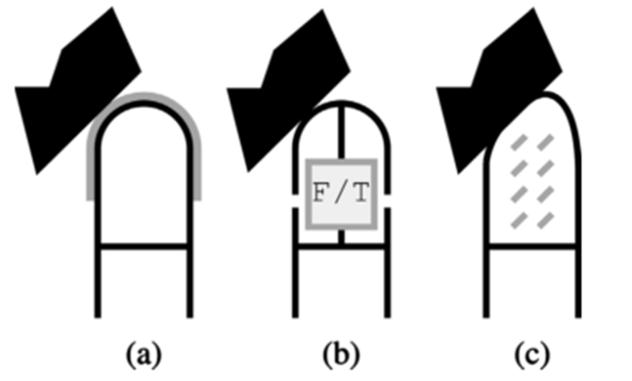
\includegraphics[width=\linewidth]{images/fingertip_sensors}
%	\caption{Different fingertip sensors: (a) tactile array - extrinsic; (b) force/torque sensor - intrinsic; and (c) fluid-filled \cite{dasu2006information}.}
%	\label{fig:fingertip_sensors}
%\end{figure}
%%ENDFIGURE

Tactile and other force and tactile sensing can provide information about mechanical properties, such as compliance, coefficient of friction, and mass, which are not perceivable through other means (e.g. vision) \cite{howe1993tactile}.
Obtaining object properties via force and tactile sensing for the purposes of succeeding in manipulation tasks has been the subject of numerous studies \cite{Heidemann2004, Detry2011, lepora2012embodied}.

The application of force and tactile sensors to many robotics problems affords new solutions that have previously been intractable via traditional, often computer vision-based methods \cite{lee1999review}.
In their 2005 review article, Tegin and Wikander \cite{tegin2005tactile} stress that, in contrast to the amount of literature on the application of vision-based solutions to robotics problems, literature on exploiting contact information (e.g. tactile) remains relatively rare.
One reason may be simply due to the lack of availability of force and tactile sensors in comparison to cameras \cite{howe1993tactile}.

While vision is arguably the dominant sense in primates, including humans, there are certain scenarios in which vision fails, such as during object occlusion or when sensory resolution is too low for a given task.
In such cases, more detailed and versatile contact information may compensate for these deficiencies.

In \cite{cutkosky2008force} the authors review techniques for processing and combining force and tactile information to develop abstract understanding of a given manipulation.
%present various layers of processing that transform raw force and tactile-sensor inputs into abstract understanding of an environment, such as object shape and contact types.
These processing techniques are shown graphically in Figure~\ref{fig:touch_id}: as raw sensory data travels from left to right, they are processed and combined to provide increasingly abstract understanding of a manipulation.
The authors state that force and tactile sensors have potential to yield the following information:
(1) object contact/no contact; 
(2) contact configuration (surface, edge, point, etc.) based on pressure-patterns; 
(3) object slip via vibrations in the grasped object, 
(4) properties (compliance, texture, friction, etc.) of an object via haptic exploration; and 
(5) feedback for control.
Given the above information, a robot can more appropriately control the force and moment on an object to accomplish the desired manipulation task.

%For object exploration, information such as local geometry, hardness, friction, texture, etc. must be obtained and integrated.
%In order to respond to events, the type and magnitude of events enacted, by for example an external agent, must be detected and properly assessed.

\subsubsection*{Example}

\begin{figure}[]
	\centering
	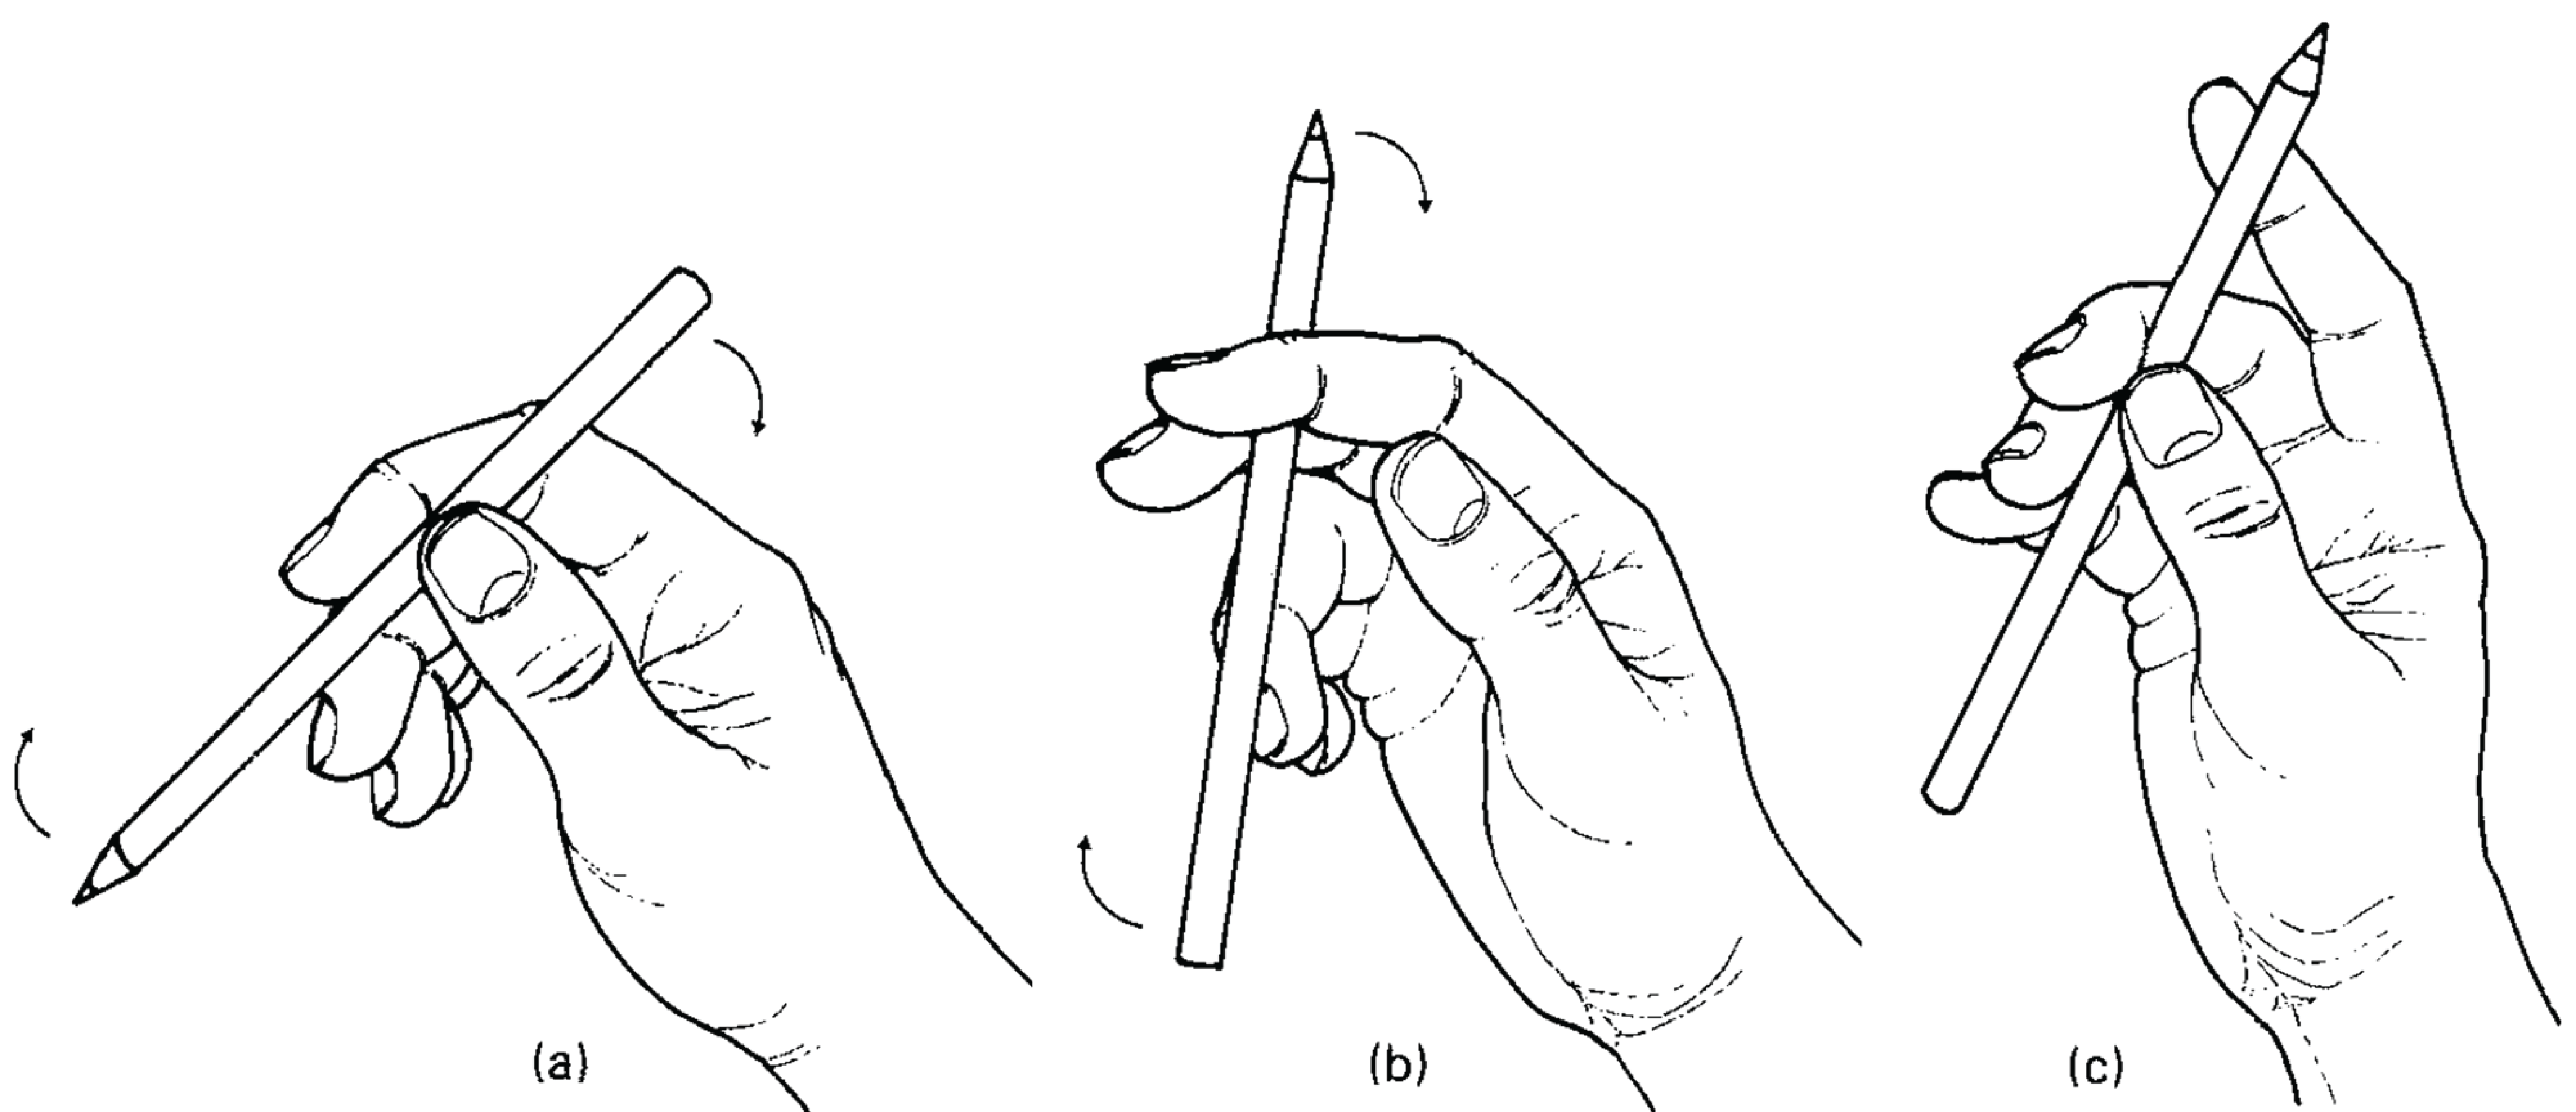
\includegraphics[width=\linewidth]{images/pen_twirling}
	\caption{Schematic drawing of the pen-twirling task. Drawings reproduced from \cite{elliott1984classification}. Use of the reproduction is by permission of the copyright owner, John Wiley and Sons.}
	\label{fig:pen_twirling}
\end{figure}

Consider the following example: how might one accomplish the task of twirling a pen end-over-end between one's fingers, as demonstrated in Figure \ref{fig:pen_twirling}? 
%What information would one use?  
The position and orientation of the object must somehow match imposed forces to maintain stability.
Successfully tracking the movement of the pen requires the knowledge of many variables, such as the configuration of one's hand, the locations and movements of contacts between the pen and one's fingers, the magnitudes of grasp forces, the contact conditions with respect to friction limits, etc.
How is it that, with enough practice, one can control all of these parameters effortlessly, even in the absense of visual feedback? 

A potential answer can be seen in Figure~\ref{fig:touch_id}: we can combine the forward kinematic model of the hand together with current finger joint angles to determine the positions and orientations of the finger tips.
When combined with force/torque measurements at the points of contact, it is possible to obtain local information of object shape, surface normal orientation, etc., which could then be combined to track the geometric pose of the object.

%Figure 2.8: 
\begin{figure}[]
	\centering
	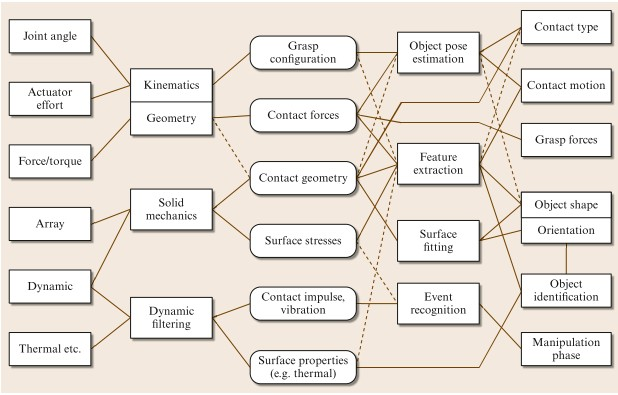
\includegraphics[width=\linewidth]{images/touch_id}
	\caption{Force and tactile sensor processing to estimate object pose \cite{cutkosky2008force}.}
	\label{fig:touch_id}
\end{figure}
%ENDFIGURE

\subsubsection*{Tactile sensing}

For robotic hands with tactile sensor arrays, such as the BarrettHand, curvature and shape information can be obtained by measuring the local curvature at each element of the sensor array \cite{cutkosky2008force}.
From there, it is possible to extract features, such as corners and edges of the object by combining local shape information from multiple sensors.
This task can be greatly enhanced if at least a partial model of the grasped object is available apriori, in which case the object can be statistically matched via surface or data fitting methods \cite{fearing1990tactile}.

The most common application of tactile information has been to classify and recognize objects from a known set based on calculated geometric information of the object from raw tactile data.
Features, such as holes, edges and corners \cite{cutkosky2008force} and object surfaces \cite{overton1981tactile} have been used and extracted from tactile array, force and/or joint sensor information.
For example, Siegel \cite{siegel1991finding} devised a way to extract object pose of a known object in a robot's grasp via joint angle and joint torque measurements.

\subsubsection*{Active Sensing}
%The common solution to obtaining object properties via force and tactile sensing is to use carefully-tailored exploratory procedures that allow the desired properties to be easily and directly predicted from the gathered data \cite{ruiz2010prediction}.
Since force and tactile sensors provide only local object information, recognition and disambiguation often require the hand to actively explore multiple areas of the object surface.
These types of strategies are referred to as active sensing.
There exist many example applications of active sensing, such as tracing object contours, measuring compliance and determining lateral extent of object surfaces.
In \cite{muthukrishnan1987edge}, the authors propose an active sensing strategy to edge-finding by exploring the surface of an object until contiguous segments of tactile array impressions are found.
In \cite{lepora2012embodied}, tactile sensors are used to discriminate shape and position of various textured cylindrical objects.
In \cite{Detry2011}, grasp affordances are obtained through exploration of the pose space of manipulable objects. 

\subsubsection*{Dynamic sensing}

The ability to detect tactile events with respect to time (e.g. object slip) is important to many manipulation tasks such as lifting fragile objects.
The challenge lies in detecting such events reliably in the presence of sensor noise.
Highly sensitive tactile sensors capable of detecting minute events can be easily thrown off by e.g. vibrations from the robot actuators or by rapid robot acceleration.
Robust dynamic event detection can be solved by comparing tactile sensor readings at and away from contact regions, or even more robustly via statistical pattern matching methods that detect the signature of particular dynamic events \cite{tremblay1993estimating}.



%TODO: FROM PAPER

\subsection{Anomaly detection in streaming data}

Since high-dimensional data streams often exhibit considerable structure, information that does not fit within this structure is most likely an anomaly, or outlier, in comparison to the vast majority of other input data.
An anomaly can be defined as an event or pattern which does not conform to some well-defined notion of normal phenomena.
Detecting the existence of anomalies within data streams is an important topic within both the data mining and machine learning communities \cite{aggarwal2003framework,kifer2004detecting,dasu2006information,yamanishi2002unifying,song2007statistical} and has far-reaching applications in such areas as fault detection, fraud detection, sensor-networks and image processing \cite{Chandola2009}.
In \cite{hornung2014anomaly}, a model-free approach is taken to find anomalies in high-dimensional sensory streams. Data collected from the robot are first passed through a PCA-based feature extractor before building models of normal operation.

%Our framework develops a model of the sensory data over the course of a prescribed motion and therefore our system can detect anomalies as data points that are in poor correspondence with predicted values.
%Knowledge of this anomaly can then initiate further action such as autonomous adaptation to cope with this anomaly or updating the current model to explain this anomaly and therefore better reflect reality.

\subsection{Dimensionality reduction}

As the number of sensors available to a system increase, the computational, storage and transmission costs in inferring information from all available sensor readings also increase.
Therefore, given a large number of sensor readings, it is important to develop a reduced set of measurements or derived features that can model desired information in a compact fashion.  
Dimensionality reduction techniques can be classified into two broad categories: (1) feature extraction and (2) feature selection.  Most feature \emph{extraction} techniques take an unsupervised \cite{ghahramani1996algorithm,saul2003think,tenenbaum2000global,hein2010unsupervised} or self-supervised \cite{angelova2007dimensionality,dahlkamp2006self,lieb2005adaptive,sofman2006improving} learning approach.  
The result is a transformed, lower-dimensional set of features that more compactly describe the underlying structure of the data.  
In contrast, feature \emph{selection} techniques, such as those based on feature similarity \cite{mitra2002unsupervised} and genetic algorithms \cite{huang2006ga}, achieve dimensionality reduction by considering only a subset of input dimensions. 
In \cite{pais2013learning}, the authors present a novel feature selection method comparing the variance of sensor readings to choose to encode either force or position information while recording user-demonstrated trajectories.

%%FIGURE (2.2)
%\begin{figure}[]
%	\centering
%	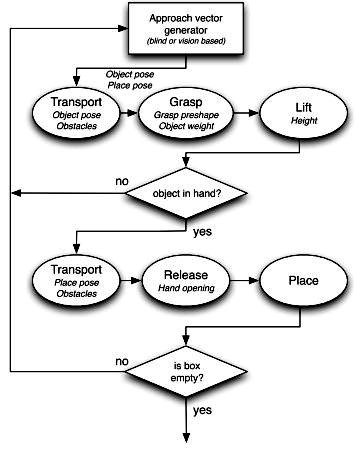
\includegraphics[width=\linewidth]{images/grasp_fsm}
%	\caption{Discrete states and transition conditions in the finite state machine that defines the empty-the-box manipulation task \cite{felip2011emptying}.}
%	\label{fig:grasp_fsm}
%\end{figure}
%%ENDFIGURE

%%Figure 2.3: 
%\begin{figure}[]
%	\centering
%	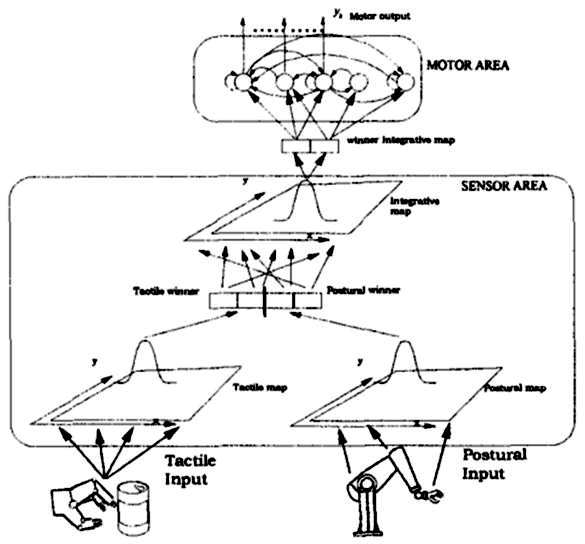
\includegraphics[width=\linewidth]{images/sensor_processing}
%	\caption{Structure of ANNs chosen by the authors as a model for human grasping \cite{leoni1998implementing}.}
%	\label{fig:sensor_processing}
%\end{figure}
%%ENDFIGURE

%%Figure 2.4: 
%\begin{figure}[]
%	\centering
%	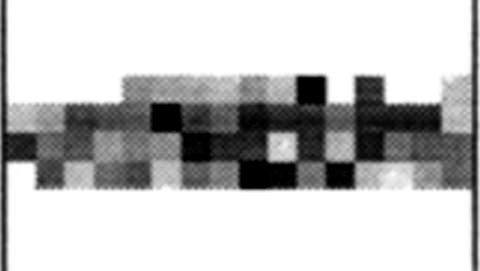
\includegraphics[width=\linewidth]{images/tactile_input}
%	\caption{Example tactile image during the rolling-pin task by planar robot finger equipped with tactile sensor array in \cite{sikka1994tactile}.
%Darkness indicates pressure intensity.}
%	\label{fig:tactile_input}
%\end{figure}
%%ENDFIGURE

%%Figure 2.5: 
%\begin{figure}[]
%	\centering
%	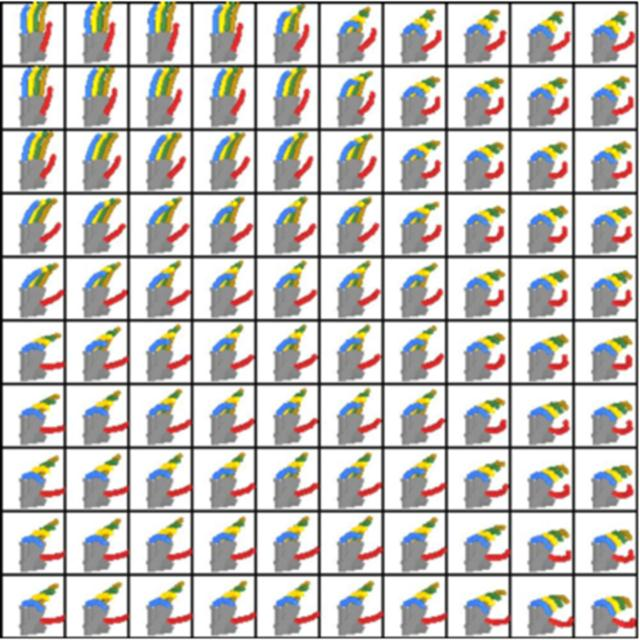
\includegraphics[width=\linewidth]{images/grasp_som}
%	\caption{Discrete grasp manifold of successful grasps based on the SOM.
%Note how similar grasp postures are organized together which results in fast queries of the experience base \cite{steffen2007experience}.}
%	\label{fig:grasp_som}
%\end{figure}
%%ENDFIGURE
%
%%FIGURE (1.8)
%\begin{figure}[]
%	\centering
%	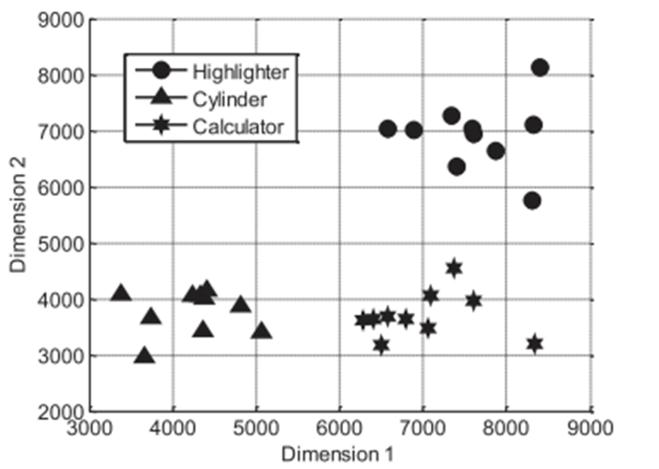
\includegraphics[width=\linewidth]{images/sensory_clustering}
%	\caption{Clusters of outputs from trained spiking neural network for certain objects \cite{ratnasingam2011spiking}.}
%	\label{fig:sensory_clustering}
%\end{figure}
%%ENDFIGURE

%%FIGURE (1.9, 2.7)
%\begin{figure}[]
%	\centering
%	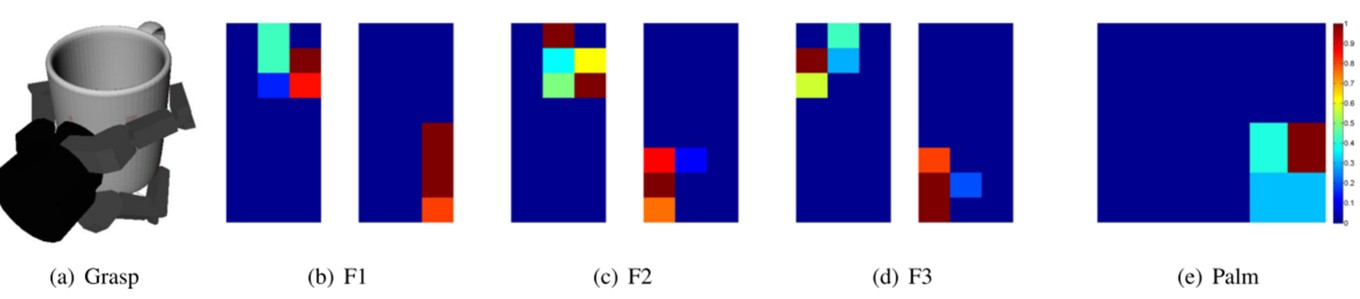
\includegraphics[width=\linewidth]{images/grasp_tactile_example}
%	\caption{Example grasp feature vector in successful grasp database: (a) shows the kinematic state of the grasp around the object, (b) (c) (d) and (e) represent the tactile feedback experienced by the first, second, third fingers and palm of the BarrettHand respectively.}
%	\label{fig:tact_example}
%\end{figure}
%%ENDFIGURE


%%FIGURE (?, 2.8)
%\begin{figure}[]
%	\centering
%	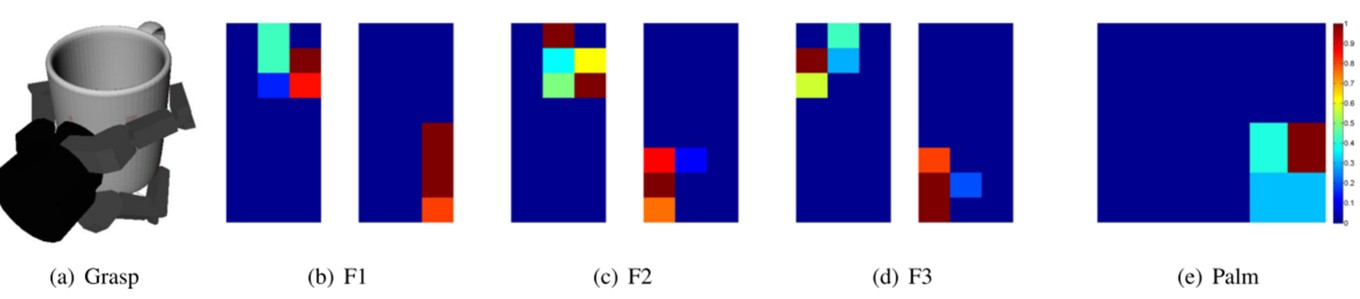
\includegraphics[width=\linewidth]{images/grasp_tactile_example}
%	\caption{Example grasp feature vector in successful grasp database: (a) shows the kinematic state of the grasp around the object, (b) (c) (d) and (e) represent the tactile feedback experienced by the first, second, third fingers and palm of the BarrettHand respectively \cite{dang2011blind}.}
%	\label{fig:tact_example}
%\end{figure}
%%ENDFIGURE

\begin{landscape}
%FIGURE (2.11, 2.12)
\begin{figure}
    %\begin{subfigure}[]{0.515\linewidth}
    %    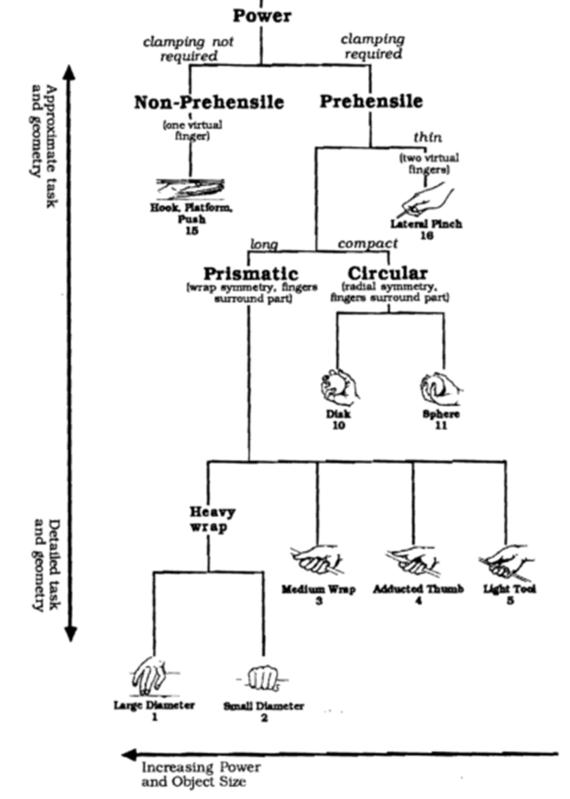
\includegraphics[width=\linewidth]{images/power_grasps}
    %    \caption{Taxonomy of power manipulation skills \cite{howe1993tactile}.}
    %    \label{fig:power_taxonomy}
    %\end{subfigure}
    %\begin{subfigure}[]{0.485\linewidth}
    %    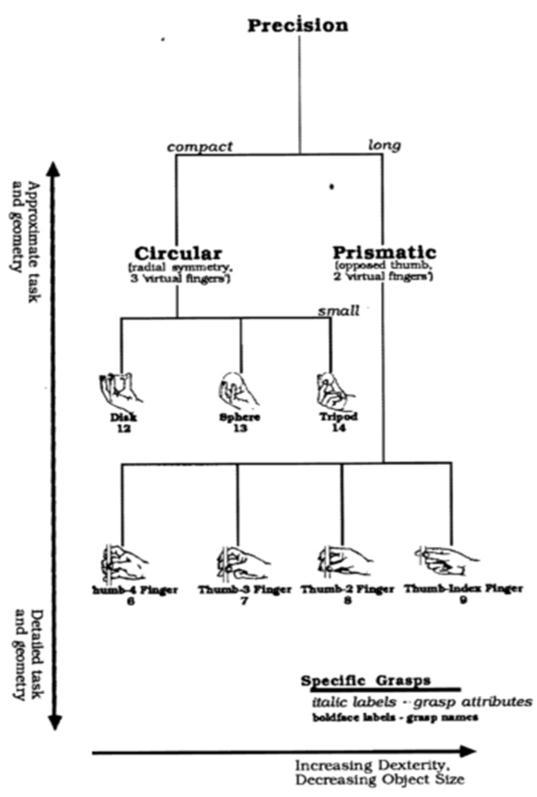
\includegraphics[width=\linewidth]{images/precision_grasps}
    %    \caption{Taxonomy of precision manipulation skills \cite{howe1993tactile}.}
    %    \label{fig:precision_taxonomy}
    %\end{subfigure}
    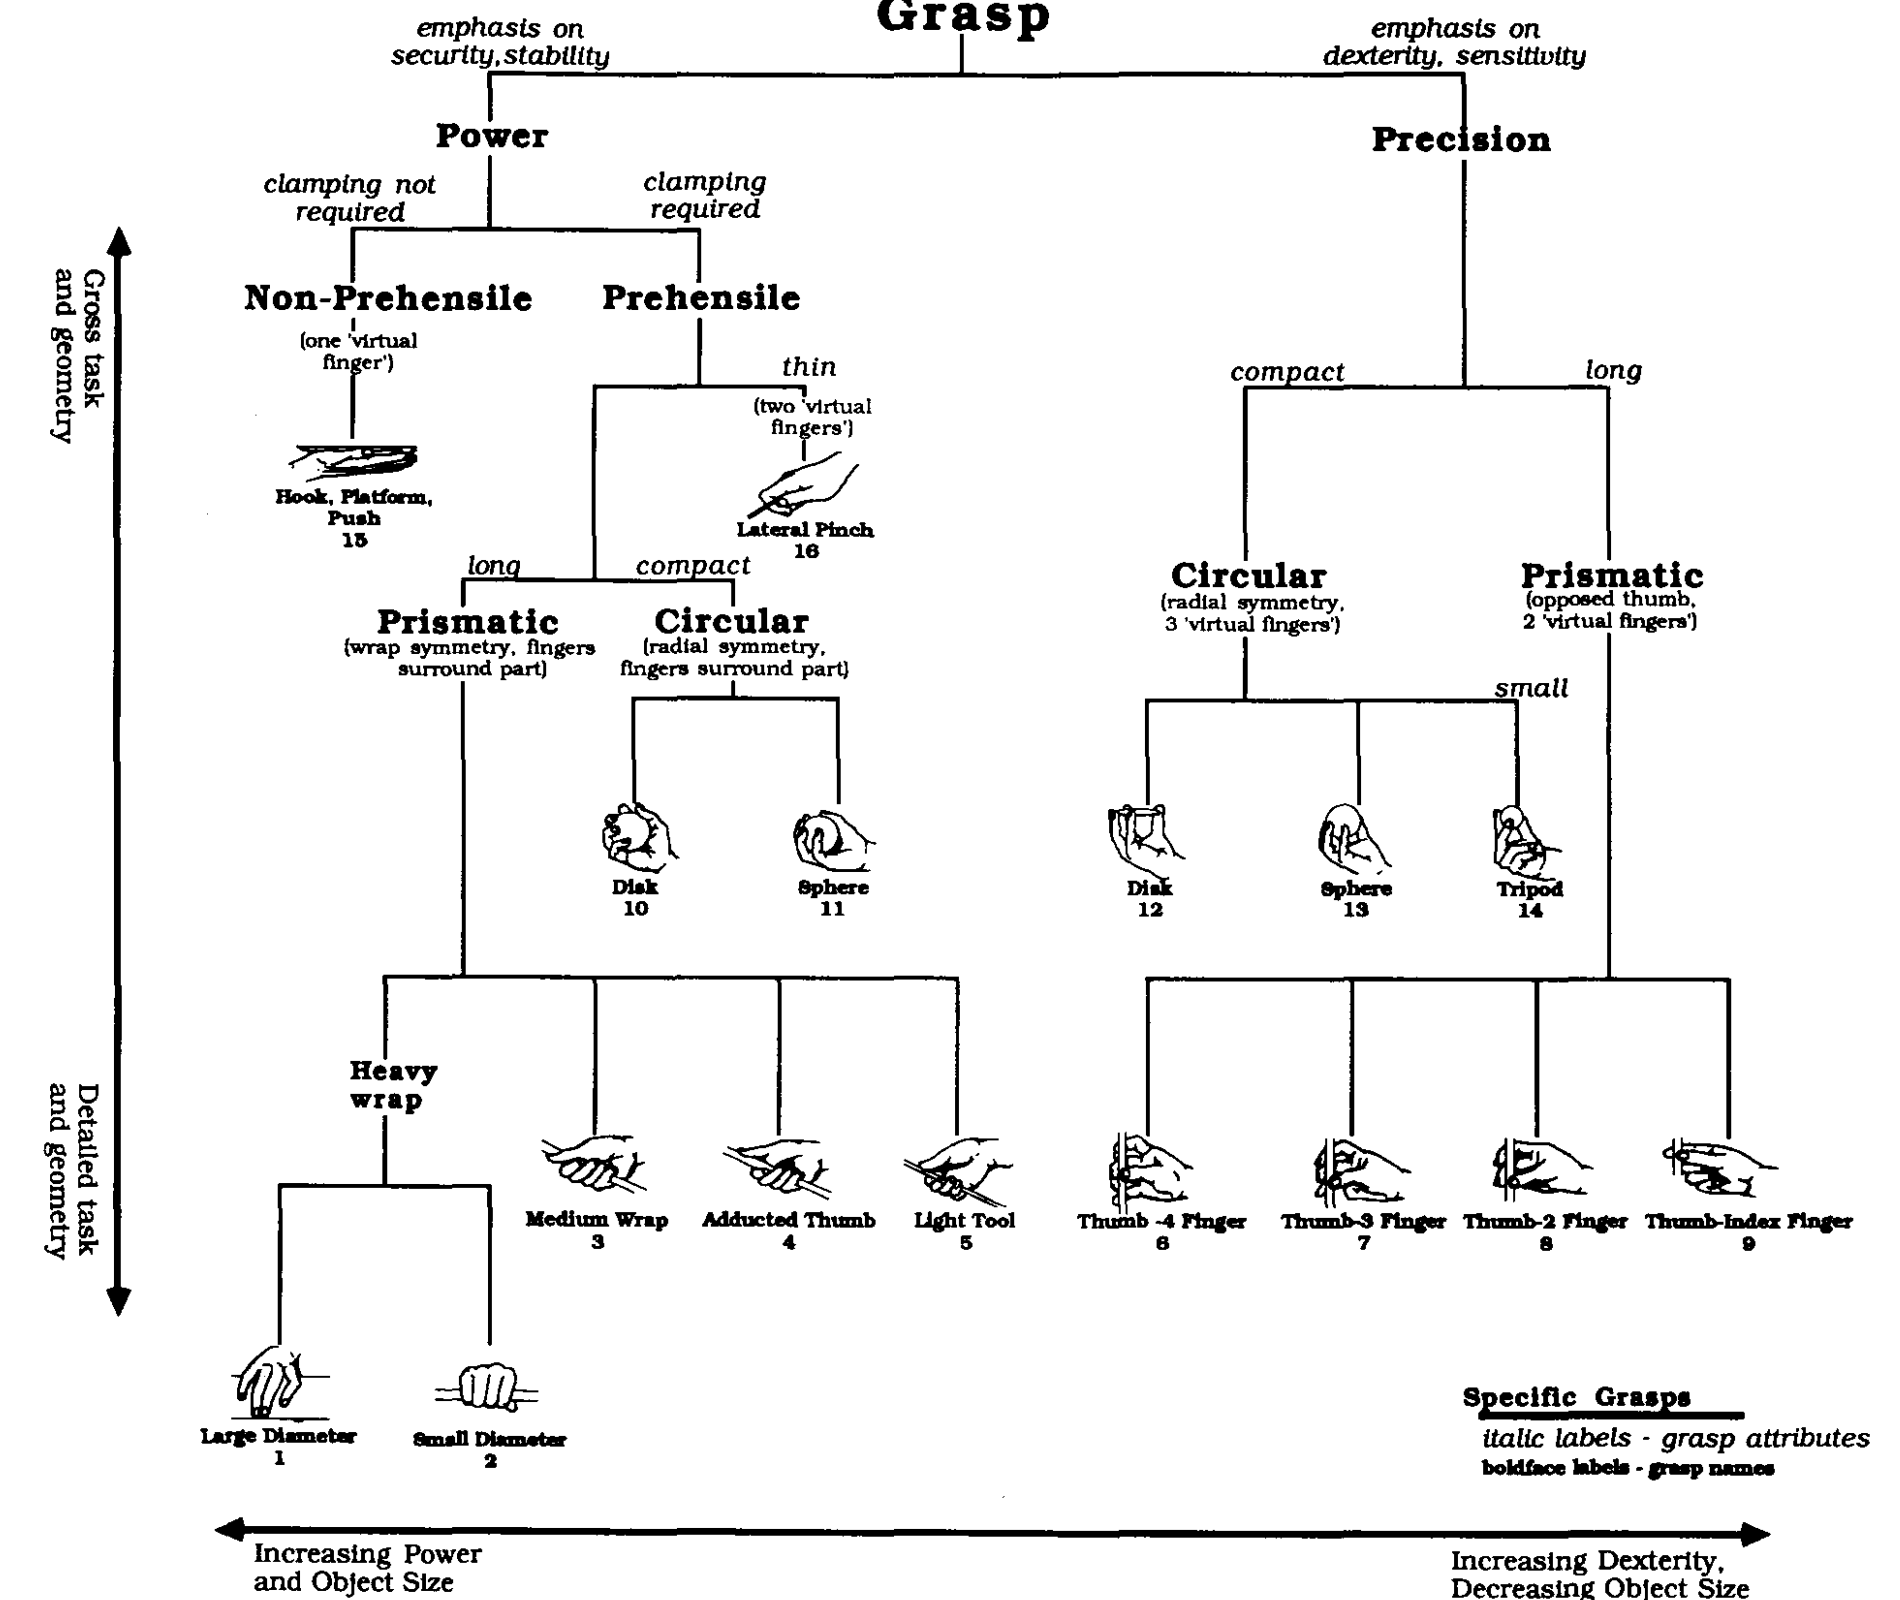
\includegraphics[width=\linewidth]{images/grasp_dichotomy}
    \caption{Dichotomy of human grasping, reproduced from \cite{cutkosky1989grasp}, \copyright 1989 IEEE. }
%Non-prehensile grasping uses gravity as a means of securing the object to the hand.
    \label{fig:grasp_dichotomy}
\end{figure}
%ENDFIGURE
\end{landscape}

\section{Neuroscience \& Physiology}

%\begin{figure}[]
%	\centering
%	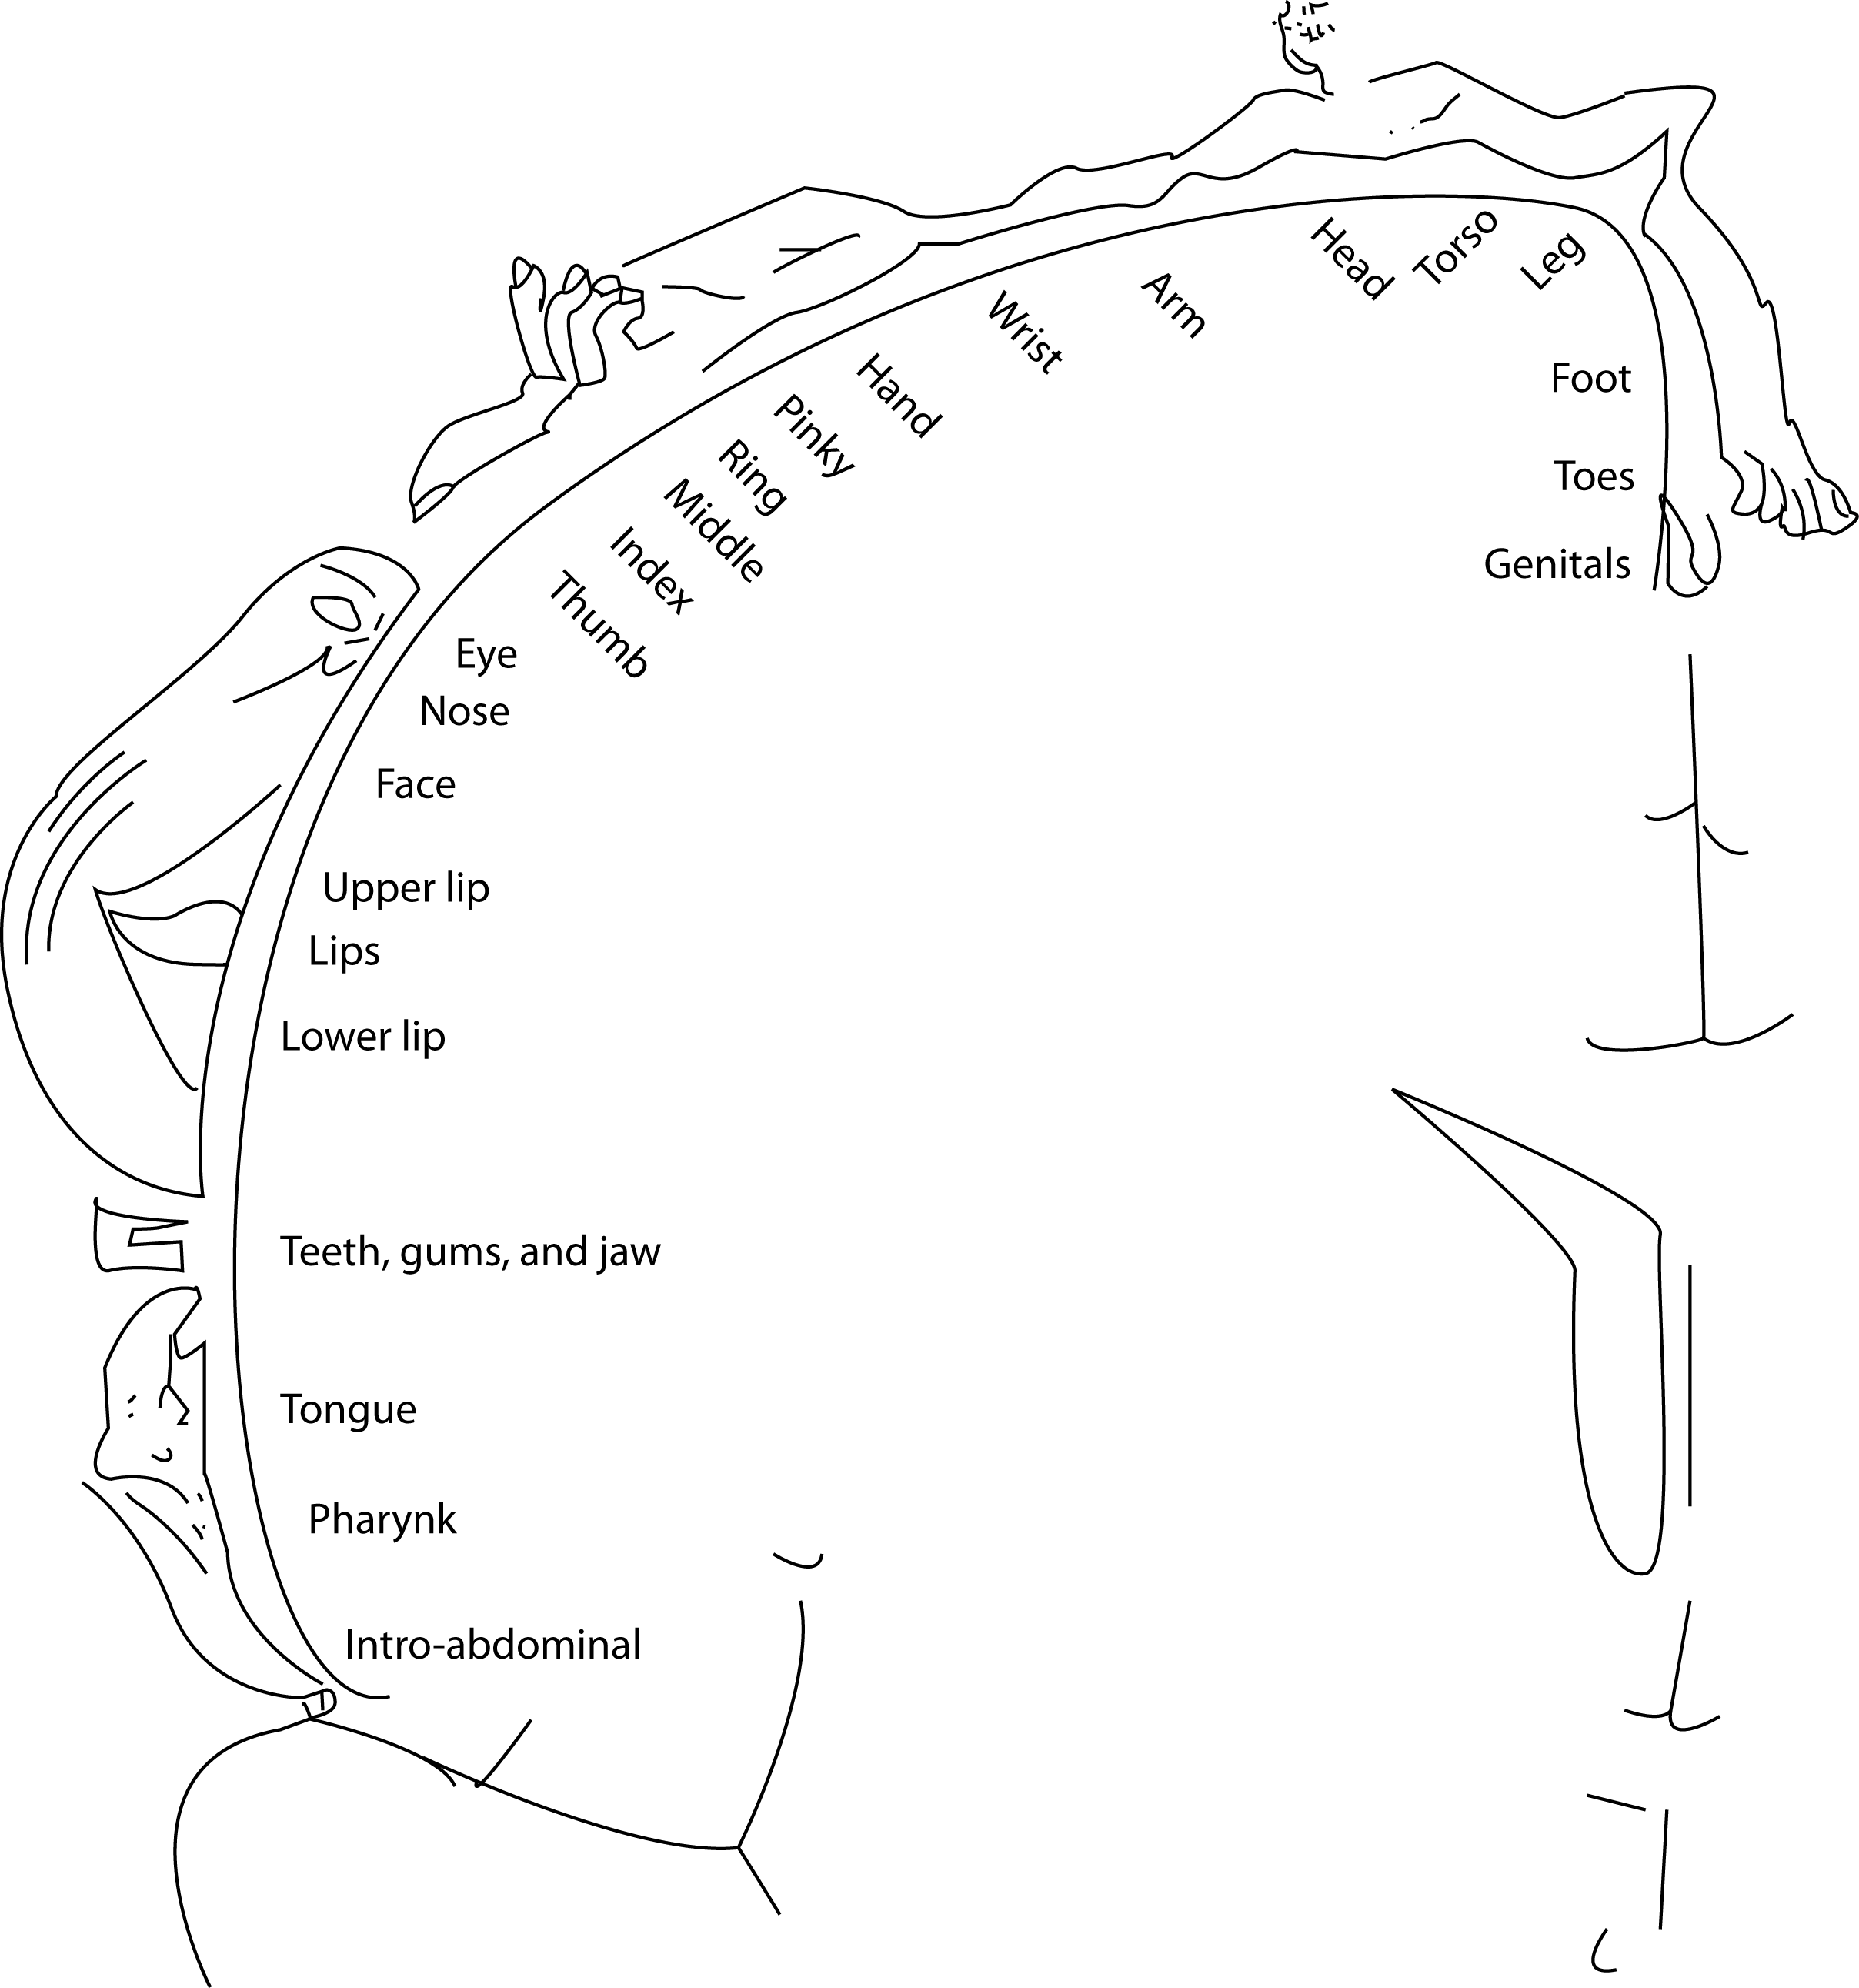
\includegraphics[width=\linewidth]{images/sensory_homunculus_penfield}
%	\caption{Human Cortical Homunculus of Penfield and Rasmussen, reproduced from \cite{penfield1950cerebral}. Permission to reproduce is pending.}
%	\label{fig:sensory_homunculus_penfield}
%\end{figure}

Studying the manipulation capabilities of humans and animals for the purpose of designing better robotic systems is a challenge.
First, it is hard to discover the precise algorithms that our brains employ.
Second, the mechanics of the human hand is highly complex and thus the algorithms our motor system employs may not be appropriate for the relatively simple mechanics of a robot.
Nevertheless, studying human manipulation can provide insight into designing more efficient and effective robotic systems.
In this section, we attempt to draw such insight by exploring the human motor system as presented in a sample of the neuroscience and physiology literature.

\subsection{Object manipulation: definitions}

In this section, we present some common vocabulary used by researchers in describing object manipulation tasks as performed by humans.

\subsubsection*{The power-precision dichotomy}

Humans employ a wide variety of manipulation skills depending on the object being manipulated.
When opening a jar, for example, a power-style grip is required to loosen the jar.
Once the lid is loose and required torque is lessened, a lighter grip is adopted for speed and precision.
This dichotomy of power/precision prehensile (i.e. grasping) activities was proposed by Napier in 1956 \cite{napier1956prehensile}.
Figure~\ref{fig:tie_rope} provides an example of these two patterns of activity in the manipulation task of tying a knot: power is required to hold the rope in place while precision is required to tie the knot. 
Cutkosky and Wright also propose a taxonomy of human grasps in \cite{cutkosky1989grasp}, breaking down the dichotomy of power/precision even further (see Figure~\ref{fig:grasp_dichotomy}).
Depending on the weight and size of the object as well as the desired dexterity of the hand, a human adopts a different style of grip.

%FIGURE (2.10)
\begin{figure}[]
	\centering
	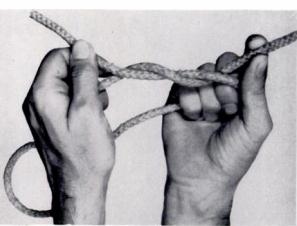
\includegraphics[width=\linewidth]{images/tie_rope}
	\caption{Tying a knot: manipulation task combining precision and power grips. Figure inspired by \cite{napier1956prehensile}.}
	\label{fig:tie_rope}
\end{figure}
%ENDFIGURE


\subsubsection*{Analytical measures of grasp quality}
The authors in \cite{cutkosky1990human} present common measures of grasp quality, which may be optimized or become part of the set of constraints with respect to a given manipulation task.
An overview of these analytical grasp-quality measures is presented in Table \ref{tbl:grasp_metrics}.
The set of ideal grasps of any object then exists within the space of grasps that satisfy all hard constraints and optimize important soft constraints with respect to the given task.
For example, Nakamura et al search for grasps that minimize internal forces (i.e. grasping effort), subject to constraints on force closure and manipulability \cite{nakamura1987mechanics}.
According to physiological findings, humans tend to employ a similar scheme as proposed by Nakamura et al where a certain frictional safety margin is maintained \cite{ring1968paper}.

Human grasps have also been studied in terms of these analytical measures.
For example, power grasps can be thought of as having higher compliance, stability and slip resistance than precision grasps.
Power grasps also tend to have a connectivity of zero (since the fingers do not play a manipulating role).
In contrast, precision grasps have high manipulability and connectivity (of at least three and often six) \cite{cutkosky1990human}.

\begin{table}[h]
\begin{tabular}{rl}
\textbf{Metric}                       & \textbf{Description}                                                               \\ \hline
\multicolumn{1}{|r|}{Compliance}      & \multicolumn{1}{l|}{Inverse-stiffness of the object with respect to the hand}      \\ \hline
\multicolumn{1}{|r|}{Connectivity}    & \multicolumn{1}{l|}{Number of DOFs between grasped object and the hand}            \\ \hline
\multicolumn{1}{|r|}{Form closure}    & \multicolumn{1}{l|}{External forces are unable to unseat the grasped object}       \\ \hline
\multicolumn{1}{|r|}{Force closure}   & \multicolumn{1}{l|}{Object held without slipping (a.k.a. frictional form closure)} \\ \hline
\multicolumn{1}{|r|}{Grasp isotropy}  & \multicolumn{1}{l|}{Fingers are able to accurately apply force/moment to object}   \\ \hline
\multicolumn{1}{|r|}{Internal forces} & \multicolumn{1}{l|}{Kinds of internal grasp forces hand may apply to the object}   \\ \hline
\multicolumn{1}{|r|}{Manipulability}  & \multicolumn{1}{l|}{Fingers can impart arbitrary motions (i.e. connectivity = 6)}  \\ \hline
\multicolumn{1}{|r|}{Slip resistance} & \multicolumn{1}{l|}{Amount of force required before object starts to slip}         \\ \hline
\multicolumn{1}{|r|}{Stability}       & \multicolumn{1}{l|}{Tendency of grasped object to return to a spatial equilibrium} \\ \hline
\end{tabular}
\caption{Common analytical measures that may be optimized or become a part of grasp constraints \cite{cutkosky1990human}.}
\label{tbl:grasp_metrics}
\end{table}

\subsubsection*{Force vs. form closure}
A subtle yet important distinction must also be made between force closure and form closure.
Only rarely do humans adopt complete form closure of objects.
Form closure refers to grasping without the use of friction whereas force closure uses friction to keep objects seated in the hand.
An object likely requiring form closure would be for example a wet bar of soap or a slinky.

\subsubsection*{Slipping vs. crushing threshold}
While adequately large grip forces must be maintained to keep the object within a force closure grasp, exceedingly large forces are also not desirable as they cause unnecessary fatigue on the hand and may even crush fragile objects \cite{johansson1994grasp}, \cite{gorniak2010manipulation}.
Thus, grip force is constrained by both the slipping and crushing thresholds of objects (see Figure~\ref{fig:grip_crush_force} for some examples).

%Figure 2.11: 
\begin{figure}[]
	\centering
	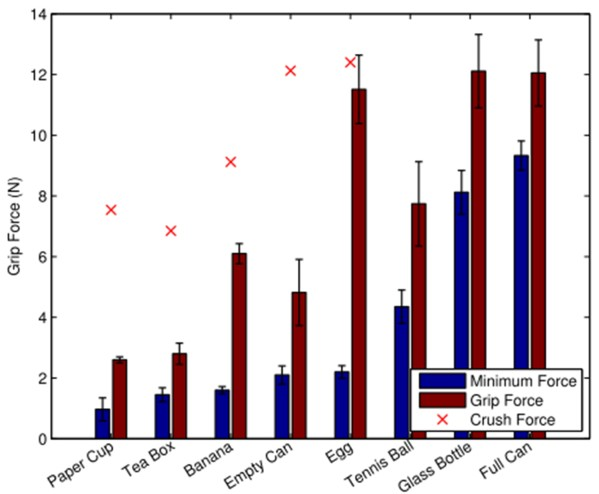
\includegraphics[width=\linewidth]{images/grip_crush_force}
	\caption{Example slipping and crushing thresholds of everyday objects \cite{romano2011human}. The difference between the required Minimum Force and observed Grip Force is known as the \emph{safety margin}.}
	\label{fig:grip_crush_force}
\end{figure}
%ENDFIGURE

The amount of force that subjects apply over and above the slipping threshold is known as the \emph{safety margin}.
The magnitude of the safety margin varies across subjects, and was found to be dependent on the dexterous manipulation skill of the subject in performing the given task \cite{Johansson1984}.

When manipulating visually fragile objects, the initial force in human subjects is lighter and their action is slower when compared to manipulating visually non-fragile objects.
Once contact with the object is made, tactile feedback complements the missing information with respect to the true fragility of the object. 
Subjects can then properly carry out the planned action \cite{chinellato2008visual}.
Accurate predictions are crucial however due to the relatively slow response rate of corrective actions \cite{johansson2009coding}.

%Information on objects involved can be predicted as well.
%If grasp stability errors occur, real-time corrective actions are taken.

\subsection{Force and tactile sensing}
\label{touch_sensing}
The elements of the human sense of touch can be broken up into two distinct categories: proprioceptive and tactile.
Proprioceptive sensing refers to the perception of limb motion and forces using internal receptors, such as muscle spindles (responding to changes in muscle length), tendon organs (measuring muscle tension), and cutaneous afferents (reacting to skin deformations around the joints) \cite{johansson2009coding}.
Proprioceptive receptors within the joints of the hand are also present, which report joint angles, forces and torques \cite{howe1993tactile}.
Tactile sensing deals with the perception of contact information with receptors beneath the surface of the skin \cite{vallbo1984properties}.

Actuation of the hand is imparted by muscles in the forearm through transmission of tension by tendons passing through the wrist.
It has been shown that due to dynamics of transmission such as friction, backlash, compliance and inertia, accurate control of endpoint position and forces based on proprioceptive signals alone is difficult \cite{kaneko1991new}.
Thus, tactile afferents are essential for fine-grained mechanical measurements at contact locations \cite{Johansson1984}.

Tactile afferents have received much attention in the physiology and neuroscience literature; a comprehensive summary of which may be found in \cite{vallbo1984properties} and, more recently in \cite{johansson2009coding}.
There are in total four specialized types of mechanoreceptive nerve endings within the skin of the human hand, each of which can be categorized as having large or small active areas (Type I and Type II respectively) and responding or not responding to static stimuli (SA for slowly adapting and FA for
fast adapting, respectively).
See Figure~\ref{fig:tactile_afferents} for a description of each of these types.
It has been calculated that a total of 17,000 specialized mechanoreceptors exist in the grasping surfaces of the human hand \cite{johansson2009coding}.
In addition, there are free nerve endings that are sensitive to thermal and pain stimuli \cite{howe1993tactile}.

%Figure 2.10: 
\begin{figure}[]
	\centering
	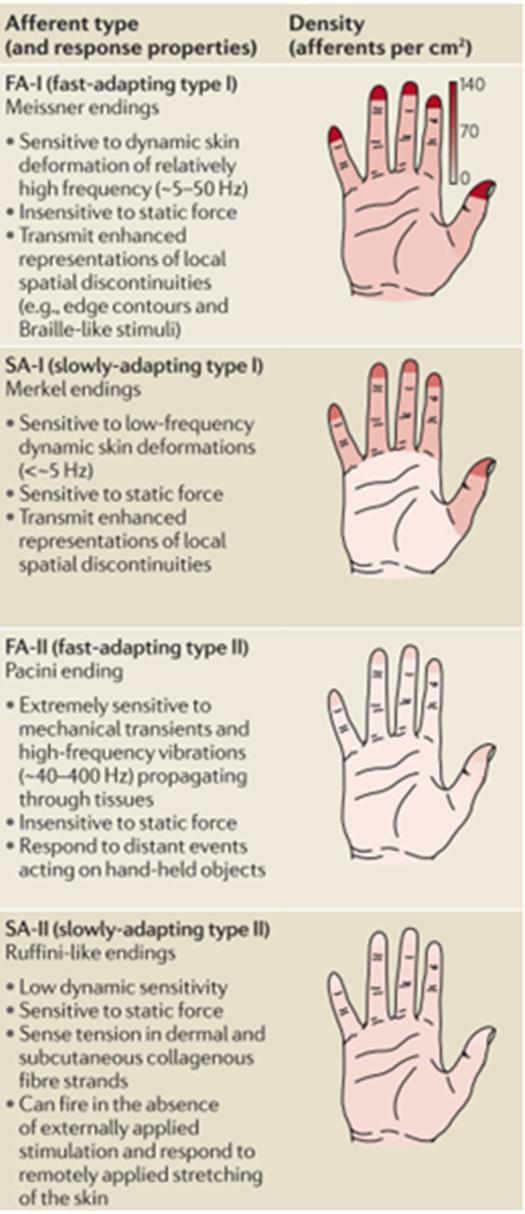
\includegraphics[width=0.7\textwidth]{images/tactile_afferents}
	\caption{Characteristic of tactile afferents within human fingertip skin.
Reproduced from \cite{johansson2009coding}. Permission to reproduce is pending. Permission to reproduce is pending.}
	\label{fig:tactile_afferents}
\end{figure}
%ENDFIGURE

\subsection{High-level processes}
\label{high_level_processes}

In addition to low-level tactile and proprioceptive processing, the mammalian central nervous system performs many high-level processes such as prediction, planning and memory.
These processes support, guide, and organize our more primitive manipulative functions to accomplish more complex manipulation tasks.

\subsubsection*{Prediction}

In \cite{johansson1994grasp}, the authors preclude that the magnitude of fingertip forces imposed on objects are determined by at least two high-level control processes: (1) anticipatory parameter control (APC) and (2) post-contact control.
The authors model APC as a feedforward controller that uses predictions of critical characteristics of the object (weight/friction/initial condition, etc.) based on the results of previous object manipulation experience.
Following contact with the object, sensory information can be extracted to (1) modify motor commands automatically; (2) update sensory memories for APC; (3) inform central nervous system of the completion of subgoals comprising a task; and (4) trigger subsequent subgoals.
The central nervous system monitors specific, expected events and produces control signals appropriate to each subgoal.
In contrast to feedback controllers, this feedforward, sensor-driven control strategy predicts appropriate control output several steps in advance.
Slips are avoided and force across digits is coordinated by independent control mechanisms based on local sensory information.

\subsubsection*{Planning}

Planning plays an important role in anticipating future events as well.
In \cite{johansson2001eye}, Johansson, et al. demonstrate the importance of eye-hand coordination during manipulation tasks.
Subjects' gaze were tracked during a block-stacking task.
It was found that their gaze played an important role in planning each pick-and-place action.
The authors then further propose and demonstrate in \cite{flanagan2003action} the direct matching hypothesis, which predicts that subjects will unconsciously produce eye movements when observing a familiar action as if they were performing the task themselves.
%This suggests deep coupling between gaze and object manipulation capabilities.

\subsubsection*{Supramodal processing}

In a study conducted by Bicchi et al \cite{scilingo2004perception}, it was found that the V5/MT cortex (the same area in the brain that responds to optical flow) is activated during tactile-flow perception, i.e. when dynamic movement is detected via tactile afferents.
This is consistent to other findings that there exists a supramodal, or multi-modal, organization of regions in the brain involved in both tactile-flow and optical-flow processing \cite{flanagan2006control}.
In another study by Bicchi et al \cite{bicchi2003haptic}, it was found that certain experiments could fool the subjects' tactile flow processing in the brain through tactile illusions, much the same way that optical-flow processing can be fooled, which is known as the \emph{aperture problem}.

\subsubsection*{Action-phase control strategies}

Findings by Johansson et al. indicate that, during certain manipulation tasks, the human motor system functions as a sort of state machine that transitions based on sensory predictions and sensory inputs.
These states, or \emph{action-phases}, are defined as sequences of specific sensory events that are each linked to subgoals comprising a given task \cite{johansson2009coding}.

Action-phase goals are evaluated by matching patterns in tactile afferent signals.
For example, grasp contact – a required action-phase subgoal for many manipulation tasks – detects patterns in SA-I and FA-II afferent inputs.
Combinations of certain afferents provide information such as contact timing, location, force intensity and direction.
Contact location is defined as the spatial center of all afferents involved in the overall signal.
Force intensity is characterized by the number of afferents involved as well as the firing rates of each.
Patterns of activity in combinations of afferents give us the direction of the detected contact force.

\subsubsection*{Dexterity}

Once a grasp is attained, adequate force within the friction cone of the object must be imposed to retain force closure.
Dexterity is then defined as the ability to adapt the balance of grip and load forces to object surface properties \cite{howe1993tactile}.
Dexterous manipulation abilities are attributed mainly to tactile afferents since a loss in these abilities is experienced during digital anesthesia \cite{Johansson1984}.

\subsubsection*{Object identification}

Tactile afferents during initial contact also provide object surface property information, which is frequently combined with visual cues and/or sensory memories to develop abstract understanding.
Reactions of FA-I, SA-I and SA-II afferents to object surface are used to determine object surface properties.
For example, FA-I afferents react more strongly to slippery surfaces \cite{burstedt1997coordination}.

\subsubsection*{Filtering noise}

Robust processing of tactile afferent information is attributed to the brain's innate ability to detect coincidence: a phenomenon in which its central neurons receive synchronous input spikes from many distinct tactile afferents \cite{hopfield1995pattern}.
Therefore, noise in the environment, i.e. information unrelated to the current focus of attention, can be characterized by input spikes which do not arrive at the brain at the same precise moment in time as input deemed valuable to the current task.





%\subsection{Non-prehensile manipulation} 
%
%This thesis is primarily concerned with non-prehensile manipulation tasks, as pioneered by Lynch and Mason \cite{lynch1999dynamic}. 
%Non-prehensile manipulation has seen relatively little attention in robotics literature despite occupying a large part of the manipulation spectrum.
%This may be attributed in part due to the difficulties of developing good models for non-prehensile object manipulation \cite{Lynch1998}.  
%Knowledge of friction, mass, and compliance are important for manipulation tasks \cite{howe1993tactile}.  
%In contrast, we develop a data-driven approach for identifying unknown dynamic properties.


%%%%

%Since our approach develops implicit models that are automatically learned by the system, developing complex apriori dynamical models of the interactions between the object and the robot is rendered redundant. %TODO: a bit too strong?

%In \cite{Pastor2011}, a robot learns the trajectory required to grasp an object through kinesthetic teaching and records expected sensory data streams to increase the likelihood of subsequent task success in light of small environmental perturbations. 
%In our work, we focus on gaining deeper insight into the changing environment so that the robot can succeed even when large perturbations are experienced.

%In \cite{Heidemann2004}, the authors evaluate time-series' of 2D tactile pressure profiles for object recognition. 
%%%%
%%%%%%%%%%%%%%%%%%%%%%%%%%%
